\subsection{Serie 9}%
\label{sub:serie_9}

\paragraph{Aufgabe 1}%
\label{par:serie_9_aufgabe_1}

Betrachten Sie ein wiederholtes Gefangenendilemma mit Stufenspiel
\begin{center}
  \begin{tabular}{ccc}
    & $C$ & $D$\\
    \cmidrule{2-3}
    $C$ & $A,A$ & $C,D$\\
    \cmidrule{2-3}
    $D$ & $D,C$ & $E,E$\\
    \cmidrule{2-3}
  \end{tabular}
\end{center}
wobei $C<E<A<D \in \RealNumbers$.
Ferner sei der Diskontierungsfaktor gegeben durch $δ \in (0,1)$.
Die Auszahlungen der Spieler im wiederholten Spiel sei die Summe der abdiskontierten
Gegenwartswerte der im aktuellen und in allen zukünftigen Stufenspielen erzielten
Nutzenwerte.

Bestimmen Sie den kleinsten Wert von $δ$, so dass es ein Gleichgewicht gibt,
in dem entlang des Gleichgewichtspfades immer $C$ gespielt wird.
Geben Sie die komplette, verwendete Gleichgewichtsstrategie an.

\paragraph{Aufgabe 2}%
\label{par:serie_9_aufgabe_2}

Betrachten Sie folgendes Spiel:
\begin{center}
  \begin{tikzpicture}
    \fill (0,0) circle (2pt) node [above left] {1};
    \fill (-1.5,-2) circle (2pt) node [above left] {2};
    \fill (1.5,-2) circle (2pt) node [below] {$0,0$};
    \fill (-3,-4) circle (2pt) node [above left] {1};
    \fill (0,-4) circle (2pt) node [below] {$0,2$};
    \fill (-4.5,-6) circle (2pt) node [below] {$1,2$};
    \fill (-1.5,-6) circle (2pt) node [below] {$2,1$};

    \draw (-4.5,-6)
      -- (-3,-4)
      node [midway, above left] {$L$}
      -- (-1.5,-6)
      node [midway, above right] {$R$};
    \draw (-3,-4)
      -- (-1.5,-2)
      node [midway, above left] {$\ell$}
      -- (0,-4)
      node [midway, above right] {$r$};
    \draw (-1.5,-2)
      -- (0,0)
      node [midway, above left] {$A$}
      -- (1.5,-2)
      node [midway, above right] {$B$};
  \end{tikzpicture}
\end{center}
\begin{enumerate}
  \item Bestimmen Sie alle Nash-Gleichgewichte in reinen Strategien.
  \item Bestimmen Sie alle teilspielperfekten Nash-Gleichgewichte.
  \item Bestimmen Sie alle perfekten Nash-Gleichgewichte
    (\emph{trembling hand perfect NE})
\end{enumerate}

\subparagraph{Lösung}%

\begin{enumerate}
  \item Wir betrachten das Spiel in der Normalform:
    \begin{center}
      \begin{tabular}{cccc}
        & & \multicolumn{2}{c}{Spieler 2}\\
        & & $\ell$ & $r$\\
        \cmidrule{3-4}
        \multirow{4}{*}{Spieler 1}
        & $AL$ & $1,\underline{2}$ & $\underline{0},\underline{2}$\\
        \cmidrule{3-4}
        & $AR$ & $\underline{2},1$ & $\underline{0},\underline{2}$\\
        \cmidrule{3-4}
        & $BL$ & $0,\underline{0}$ & $\underline{0},\underline{0}$\\
        \cmidrule{3-4}
        & $BR$ & $0,\underline{0}$ & $\underline{0},\underline{0}$\\
        \cmidrule{3-4}
      \end{tabular}
    \end{center}
    Damit gilt $\text{NGG} = \{(AL,r), (AR,r), (BL,r), (BR,r)\}$.

  \item Es gilt:
    \begin{center}
      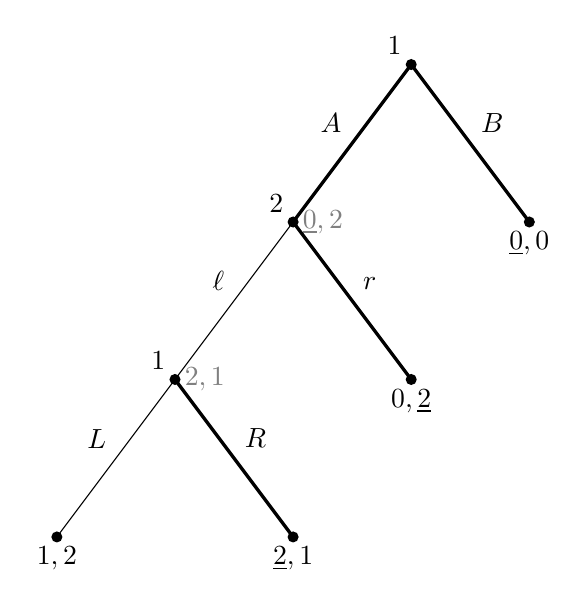
\begin{tikzpicture}
        \fill (0,0) circle (2pt) node [above left] {1};
        \fill (-1.5,-2) circle (2pt)
          node [above left] {2}
          node [right, gray] {$\underline{0},2$};
        \fill (1.5,-2) circle (2pt) node [below] {$\underline{0},0$};
        \fill (-3,-4) circle (2pt)
          node [above left] {1}
          node [right, gray] {$2,1$};
        \fill (0,-4) circle (2pt) node [below] {$0,\underline{2}$};
        \fill (-4.5,-6) circle (2pt) node [below] {$1,2$};
        \fill (-1.5,-6) circle (2pt) node [below] {$\underline{2},1$};

        \draw (-4.5,-6) -- (-3,-4) node [midway, above left] {$L$};
        \draw [very thick] (-3,-4) --  (-1.5,-6) node [midway, above right] {$R$};
        \draw (-1.5,-2) -- (-3,-4) node [midway, above left] {$\ell$};
        \draw [very thick] (-1.5,-2) -- (0,-4) node [midway, above right] {$r$};
        \draw [very thick] (-1.5,-2) -- (0,0) node [midway, above left] {$A$};
        \draw [very thick] (0,0) -- (1.5,-2) node [midway, above right] {$B$};
      \end{tikzpicture}
    \end{center}
    Damit ist $\text{SPNE} = \{(AR, r), (BR,r)\}$.
\end{enumerate}

